\section{INTRODUÇÃO}
O fechamento de vias urbanas é uma alternativas frequentemente utilizadas para atender objetivos como melhoria do tráfego, redução de acidentes ou a criação de áreas de lazer e trânsito de pedestres. Buscando diminuir o tempo de veículos parados devido ao transito, dar celeridade e desafogar o congestionamento de veículos no centro da cidade, Autarquia de Mobilidade de Caruaru (AMC) apresentou a proposta do fechamento da travessa 13 de Maio, a partir do dia 21 de novembro de 2024. O fechamento de uma via pode gerar um impacto negativo e causar transtorno a toda população, diante dessa situação é fundamental realizar uma análise robusta para avaliar os resultados do fechamento de uma via, garantindo que as alterações aplicadas em vias públicas sejam fundamentadas em dados concretos e tragam, de acordo com a análise dos dados, benefícios a população. 
Este estudo busca analisar o impacto do fechamento de uma via urbana específica, a Travessa 13 de Maio. Utilizando a metodologia do teste de hipótese, é possível verificar se há uma diferença estatisticamente significativa no comportamento do tráfego e na mobilidade da área afetada. Este teste é uma ferramenta analítica importante, capaz de fornecer evidências que justifiquem ou não, uma afirmação sobre a realidade observada. Empregando esta metodologia, o estudo se propõe a analisar as decisões tomadas pela Autarquia de Mobilidade Urbana (AMC) em relação ao impacto causado com o fechamento da travessa 13 de Maio.
\section{REFERENCIAL TEÓRICO}

\subsection{Teste de Hipótese}
O teste de hipótese, é uma metodologia estatística fundamental para a tomada de decisões baseada em dados, amplamente utilizada nas mais diversas áreas do conhecimento, como engenharia, ciências sociais, economia e saúde etc. O teste de hipótese envolve, basicamente, a verificação de uma afirmação (hipótese) sobre um parâmetro populacional, com objetivos de determinar se os dados disponíveis fornecem evidências suficientes para rejeitar ou não essa hipótese. O trabalho de  \citealp{naghettini2007hidrologia} relata que testar uma hipótese é recolher evidências nos dados amostrais que justifiquem a rejeição ou não de uma certa hipótese sobre um parâmetro populacional ou sobre a forma de um modelo  distributivo, levando em conta as probabilidades de serem tomadas decisões incorretas. 


O processo envolve a formulação de duas hipóteses contrapostas: a hipótese nula (\( H_0 \)) e a hipótese alternativa (\( H_1 \)). A hipótese nula (\( H_0 \)) representa uma situação de “não efeito” ou “não diferença”, sendo assim, assume-se que não existe relação entre as variáveis ou que o parâmetro populacional é igual a um valor específico. Já a hipótese alternativa (\( H_1 \)) sugere que existe uma diferença significativa, ou que o parâmetro populacional apresenta um valor diferente daquele especificado na hipótese nula (\( H_0 \)). O teste é realizado através de uma amostra de dados, e o objetivo é determinar se a amostra oferece evidências suficientes para rejeitar a hipótese nula (\( H_0 \)) em favor da hipótese alternativa (\( H_1 \)). 

A realização do teste de hipótese é estruturada em quatro etapas principais: 
\begin{enumerate}
    



\item Formulação da hipótese: define-se a hipótese nula (\( H_0 \)) é a hipótese alternativa (\( H_1 \)). 

\item  Escolha do nível de significância(\(\alpha\)): Determina-se a probabilidade de cometer um erro tipo I (rejeitar  \( H_0 \) quando ela é verdadeira) comumente, utiliza-se um nível de 5\% (\(\alpha\) = 0,05).

\item Cálculo do valor do teste estatístico: Dependendo do tipo de dados e da distribuição da amostra, o valor do teste pode ser, por exemplo, uma estatística, t, z ou qui-quadrado. 
\item Conclusão: Compara-se o valor do teste com a distribuição de referência (distribuição normal, t, etc) e decide-se se rejeita ou não a hipótese nula (\( H_0 \)). Caso o valor-p (probabilidade de obter resultados tão extremos quanto os observados, assumindo que a \( H_0 \) seja verdadeiro) seja menor que o nível de significância, rejeita-se \( H_0 \). 
\end{enumerate}
Existem vários tipos de testes de hipóteses, como os testes de duas caudas (quando se espera uma diferença em qualquer direção) e os testes de uma cauda (quando se espera uma diferença em uma direção específica). Outro aspecto importante são os erros em testes de hipóteses: o erro tipo I ocorre quando se rejeita a hipótese nula (\( H_0 \)) quando ela é verdadeira, e o erro tipo II ocorre quando se aceita a hipótese nula (\( H_0 \)) quando ela é falsa. 

O tamanho da amostra desempenha um papel fundamental na robustez dos testes. As amostras maiores tendem a fornecer estimativas mais precisas e aumentar o poder do teste, logo, a probabilidade de rejeitar a hipótese nula (\( H_0 \)) quando ela é de fato falsa. Sendo assim, a escolha adequada do tamanho amostral é essencial para evitar ambos os tipos de erro. 

Os testes de hipóteses são amplamente utilizados na prática científica, para fornecer uma base quantitativa nos processos decisórios. Porém, é importante considerar que mesmo que uma hipótese nula (\( H_0 \)) seja rejeitada, isso não prova que a hipótese alternativa seja verdadeira de maneira absoluta, apenas que ela é mais confiável com base nos dados observados. 
\section{Metodologia}
A AMC forneceu os dados de volume de veículos que passam por cada semáforo a cada hora na cidade, de novembro de 2023 a dezembro de 2024. A fim de identificar o impacto do fechamento da travessa foi filtrado os meses de novembro e dezembro dos dois anos analisados. Na imagem \ref{fig:mapa} abaixo podemos ver o mapa de onde a travessa se localiza.  

\begin{figure}[H]
    \centering
    \caption{Mapa da Travessa 13 de maio}
    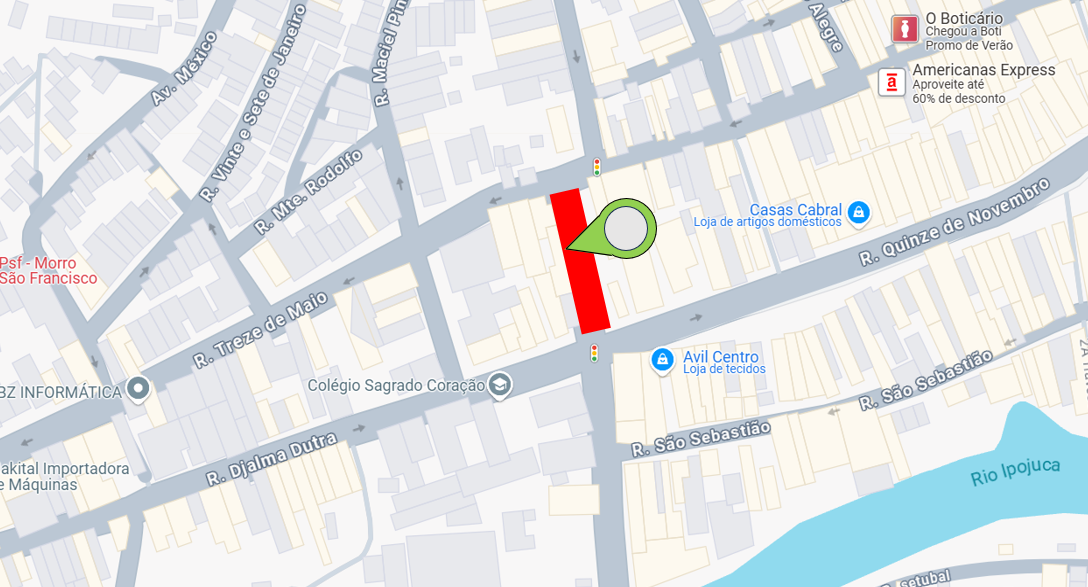
\includegraphics[width=0.7\linewidth]{Imagens/map.png}
    {\footnotesize \\Fonte: OpenStreetMap}
    \label{fig:mapa}
\end{figure}
No local há dois semáforos , um cuida da junção da Rua Djalma Dutra com a Rua Quinze de novembro e outro Rua Djalma Dutra com Av. Lourival José da Silva. Fisicamente eles ficam no mesmo local. Esses foram os equipamentos selecionados para a analise nesse trabalho. Além disso, foi selecionado os horários das 7:00 as 18:59. Na imagem abaixo podemos ver  o volume de veículos nesses horários.
\begin{figure}[H]
    \centering
    \caption{Volume por horário}
    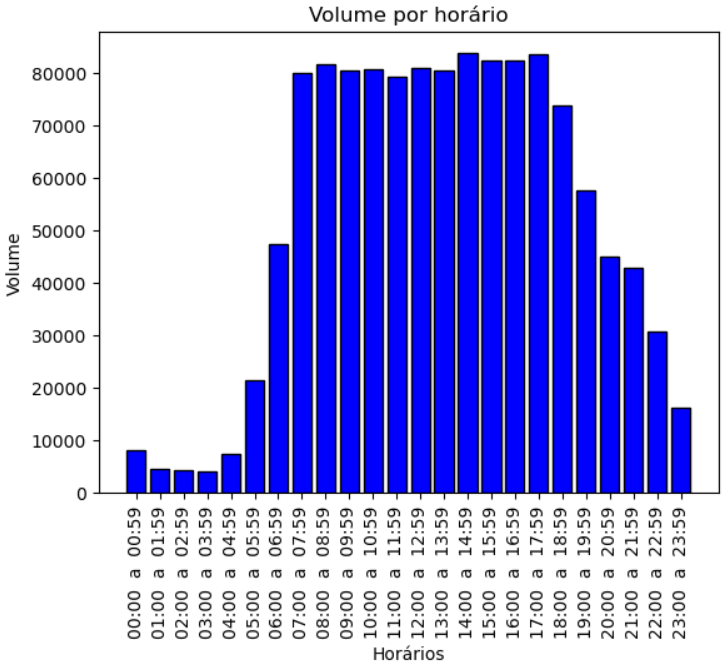
\includegraphics[width=0.7\linewidth]{Imagens/volume.png}
    {\footnotesize\\ Fonte: o autor}
    \label{fig:volume}
\end{figure}
Em especial foi dada atenção aos horários de 7:00 as 7:59, 12:00 as 12:59 e 17:00 as 17:59, esses são normalmente os horários das pessoas irem ao trabalho/escola, almoçar e voltar do trabalho/escola para casa, respectivamente.
O controle foi feito comparando se há aumento significativo do fluxo nos demais semáforos no mês de dezembro. Assim podemos identificar se houve um aumento generalizado na cidade ou não.

\section{Resultados E Discussão}
\subsection{Antes da alteração}
Baseado nos dados obtidos de volume dos sinais, comparou-se os dados de do dia 1 ao dia 21 de novembro dos anos de 2023 e 2024 para evitar efeitos de sazonalidade. Desconsiderando Sábados e Domingos. Assim, as hipóteses são:
\begin{equation*}
    \begin{aligned}
 \quad H_0 : u_1=u_2\\
 \quad H_1 : u_1\neq u_2
    \end{aligned}
\end{equation*}
sendo \(u_1\) a média do fluxo de veículos no começo de novembro de 2023, e \(u_2\) para 2024. Assim, podemos verificar se houve mudança significativa no fluxo nesse mesmo período em dois anos diferentes. Fazendo um teste T de student para amostras dependentes temos os resultados nas imagens \ref{fig:t7},\ref{fig:t12} e \ref{fig:t17} para os 3 horários 7:00 as 7:59, 12:00 as 12:59 e 17:00 as 17:59 respectivamente.
\begin{figure}[H]
    \centering
    \caption{Teste de hipotese 7:00 as 7:59}
    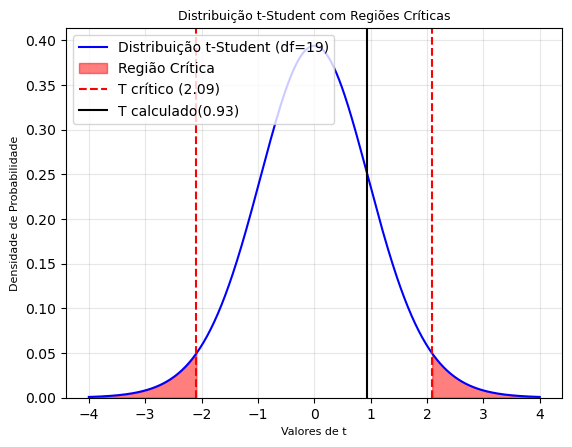
\includegraphics[width=1\linewidth]{Imagens/7.png}
    {\footnotesize\\ Fonte: o autor}
    \label{fig:t7}
\end{figure}
fazendo o mesmo teste para o horário de 12h
\begin{figure}[H]
    \centering
    \caption{Teste de hipotese 12:00 as 12:59}
    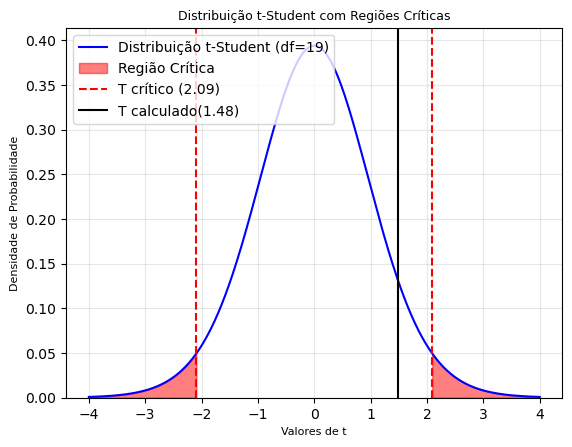
\includegraphics[width=1\linewidth]{Imagens/12.png}
    {\footnotesize\\ Fonte: o autor}
    \label{fig:t12}
\end{figure}

e as 17h
\begin{figure}[H]
    \centering
    \caption{Teste de hipotese 17:00 as 17:59}
    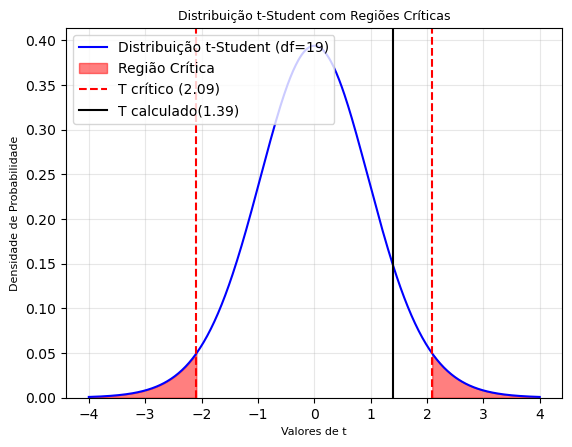
\includegraphics[width=1\linewidth]{Imagens/17.png}
    {\footnotesize\\ Fonte: o autor}
    \label{fig:t17}
\end{figure}
Nesses 3 testes não há evidências significativas para rejeitar \(H_0\), logo consideramos que não houve mudança significativa do volume de carros nas primeiras semanas de novembro de 2023 e 2024.
Na tabela \ref{tab:pvalores} abaixo há o \(P-valor\) para os testes nos demais horários.

\begin{table}[H]
\centering
\caption{P-valores do teste de hipótese por horário.}
\begin{tabular}{cc}
\hline
\textbf{\(P\)-valor} & \textbf{Horário} \\ \hline
0,189 & 06:00 a 06:59 \\
0,363 & 07:00 a 07:59 \\
0,197 & 08:00 a 08:59 \\
0,120 & 09:00 a 09:59 \\
0,187 & 10:00 a 10:59 \\
0,133 & 11:00 a 11:59 \\
0,154 & 12:00 a 12:59 \\
0,094 & 13:00 a 13:59 \\
0,212 & 14:00 a 14:59 \\
0,493 & 15:00 a 15:59 \\
0,257 & 16:00 a 16:59 \\
0,180 & 17:00 a 17:59 \\ \hline
\end{tabular}
{\footnotesize\\ Fonte: o autor.}
\label{tab:pvalores}
\end{table}




Em nenhum dos horários analisados, houve evidências o suficiente para rejeitar a hipótese nula, então podemos considerar que o volume de veículos foi igual nas primeiras semanas de novembro em 2023 e 2024.
\subsection{Após a Alteração}
A intervenção começou no dia 21 de novembro, com testes, considerando que há um tempo para os motoristas se habituarem a mudança. A analise a seguir é a comparação no mês de dezembro dos dois anos. As hipóteses são:
\begin{equation*}
    \begin{aligned}
     &H_0: u_1 \leq u_2\\
     &H_1: u_1 > u_2\\
    \end{aligned}
\end{equation*}
A hipótese nula nos testes diz se a média \(u_1\) é menor ou igual a \(u_2\), a hipótese alternativa que \(u_2\) é menor. sendo \(u_1\) a média do fluxo de veículos em dezembro de 2024, e \(u_2\) para 2023.
Fazendo um teste T de student para amostras dependentes temos os resultados nas imagens \ref{fig:t72},\ref{fig:t122} e \ref{fig:t172} para os 3 horários 7:00 as 7:59, 12:00 as 12:59 e 17:00 as 17:59 respectivamente.
\begin{figure}[H]
    \centering
    \caption{Teste de hipótese 7:00 as 7:59 em dezembro}
    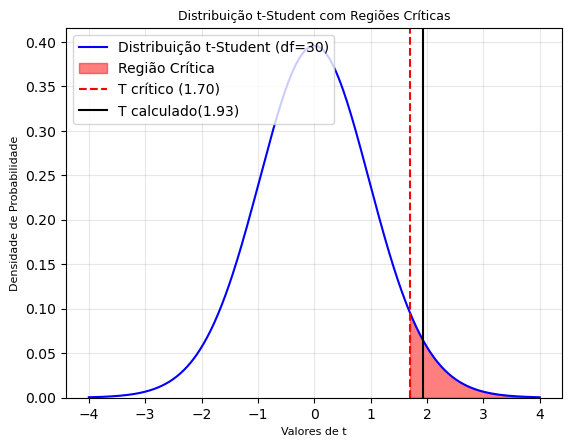
\includegraphics[width=1\linewidth]{Imagens/72.png}
    {\footnotesize\\ Fonte: o autor}
    \label{fig:t72}
\end{figure}
fazendo o mesmo teste para o horário de 12h
\begin{figure}[H]
    \centering
    \caption{Teste de hipótese 12:00 as 12:59  em dezembro}
    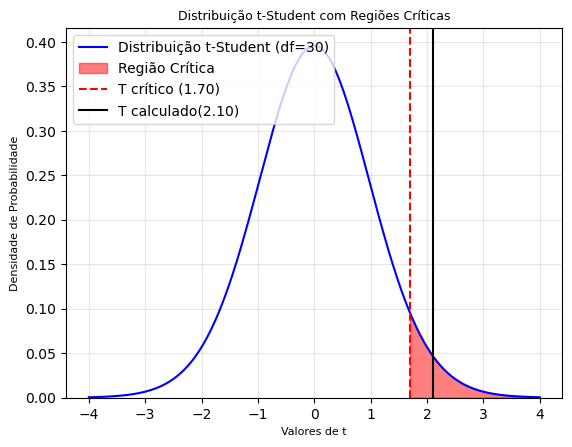
\includegraphics[width=1\linewidth]{Imagens/122.png}
    {\footnotesize\\ Fonte: o autor}
    \label{fig:t122}
\end{figure}

e as 17h
\begin{figure}[H]
    \centering
    \caption{Teste de hipótese 17:00 as 17:59  em dezembro}
    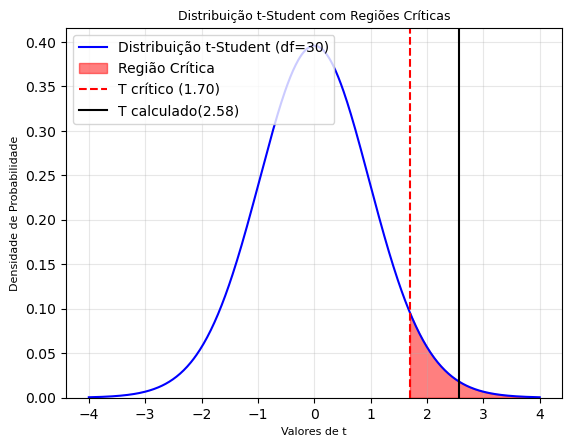
\includegraphics[width=1\linewidth]{Imagens/172.png}
    {\footnotesize\\ Fonte: o autor}
    \label{fig:t172}
\end{figure}

Nos 3 testes há evidencias o suficiente com um nível de significância \(\alpha=0,05\) que o volume de veículos em dezembro de 2024 foi maior que em 2023 no mesmo período nesses 3 horários. Na tabela a seguir há os resultados para os demais horários. 
\begin{table}[H]
\centering
\caption{P-valores do teste de hipótese por horário em dezembro.}
\begin{tabular}{cc}
\hline
\textbf{\(P\)-valor} & \textbf{Horário} \\ \hline
0,015 & 06:00 a 06:59 \\
0,032 & 07:00 a 07:59 \\
0,011 & 08:00 a 08:59 \\
0,001 & 09:00 a 09:59 \\
0,000 & 10:00 a 10:59 \\
0,001 & 11:00 a 11:59 \\
0,022 & 12:00 a 12:59 \\
0,006 & 13:00 a 13:59 \\
0,007 & 14:00 a 14:59 \\
0,005 & 15:00 a 15:59 \\
0,014 & 16:00 a 16:59 \\
0,008 & 17:00 a 17:59 \\ \hline
\end{tabular}
{\footnotesize\\ Fonte: o autor.}
\label{tab:pvalores2}
\end{table}

Com isso, há evidências estatísticas que houve um aumento do volume de carros nesses semáforos em todos os horários analisados nesse estudo. Na imagem \ref{fig:dezembro}  podemos ver que a linha de tendência do volume de carros  em dezembro por dia nos dois anos.  Podemos observar que ambas apresentam uma diminuição do volume ao passar do mês mas em 2024 mantém uma tendência maior.
\begin{figure}[H]
    \centering
    \caption{Volume em dezembro por dia}
    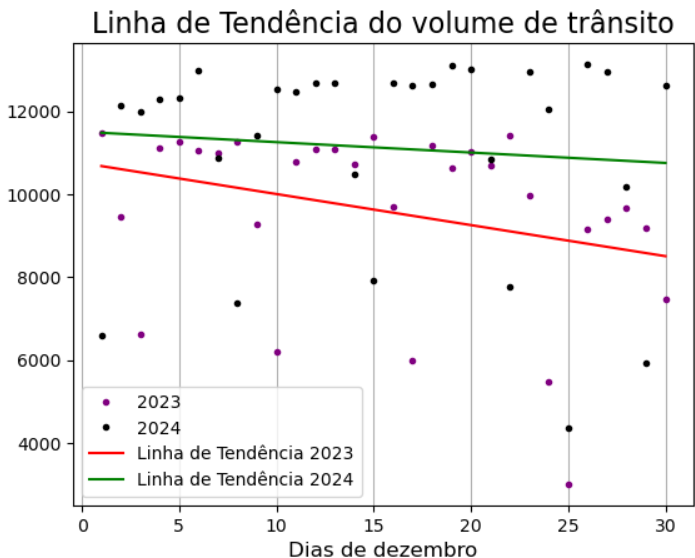
\includegraphics[width=0.7\linewidth]{Imagens/dezembro.png}
    {\footnotesize\\ Fonte: o autor}
    \label{fig:dezembro}
\end{figure}
\subsection{Outros semáforos}
Com o objetivo de identificar se o aumento no volume de veículos ocorreu em outros semáforos da cidade, foram analisados os demais equipamentos que registram o fluxo de veículos por hora. O quadro \ref{tab:enderecos} apresenta a relação dos endereços onde estão localizados esses semáforos, acompanhados de seus índices, que foram atribuídos neste trabalho como forma de simplificar a identificação e facilitar as citações.






\begin{quadro}[H]
\centering
\caption{Endereços dos demais semáforos}
\begin{tabular}{|c|l|}
\hline
\textbf{Índice} & \textbf{Endereço} \\ \hline
1  & Av. Adjar da Silva Casé \\ \hline
2  & Av. José Rodrigues de Jesus,\\ &(próximo a Motorac) \\ \hline
3  & Av. Leão Dourado \\ \hline
4  & Rua Capitão João Velho x\\& Rua Coronel Limeira \\ \hline
5  & Rua Capitão João Velho\\& x Vigário Freire \\ \hline
6  & Av. Agamenon Magalhães x\\& Rua Francisca Lira Florêncio \\ \hline
7  & Av. Agamenon Magalhães\\& (Final da Av. Agamenon) \\ \hline
8  & Av. Rui Barbosa x Avenida Caruaru \\ \hline
9  & Av. Caruaru x Av.\\& Rui Barbosa (Viaduto Boa vista) \\ \hline
10 & Av. Leão Dourado \\&(Viaduto São Francisco) \\ \hline
11 & Avenida Agamenon Magalhães x\\& Rua Gonçalves Dias \\ \hline
12 & Av. Adjar da Silva Casé\\& (Maria José I – sentido shopping) \\ \hline
13 & Avenida Manoel de\\& Freitas (Armando da Fonte) \\ \hline
14 & Avenida Caruaru x\\& Rua Santa Maria da Boa Vista \\ \hline
15 & Av. Marcionílio Francisco x Av.\\& Amazonas (Igreja da Natividade) \\ \hline
16 & Estrada para Xique Xique \\ \hline
17 & Av. Portugal x Av. Brasil \\ \hline
18 & Av. Joao Soares Machado \\ \hline
\end{tabular}
{\footnotesize\\ Fonte: o autor}
\label{tab:enderecos}
\end{quadro}

Na tabela abaixo há os \(p-valores\) dos testes T para amostras independentes com as hipóteses:
\begin{equation*}
    \begin{aligned}
     &H_0: u_1 \leq u_2\\
     &H_1: u_1 > u_2\\
    \end{aligned}
\end{equation*}
A hipótese nula nos testes diz se a média  do volume de veículos em dezembro de 2023 \(u_1\) é maior ou igual a \(u_2\) que é a média em a 2024. \(H_1\) é  que \(u_1\) é menor que  \(u_2\). Isso em cada semáforo .

% \begin{center}
% Tabela 3: \(P-\) % Título da tabela
% \end{center}
\vspace{0.5cm}
\tablehead{\hline & &   Índice \\\(P-\)Valor & Horário &do semáforo
\\ \hline}
\centering
\tabletail{\hline}
\topcaption{Testes de hipótese nos demais semáforos}
\begin{supertabular}{ccc}
0,913 & 07:00 a 07:59 & 1 \\
1,000 & 12:00 a 12:59 & 1 \\
0,967 & 17:00 a 17:59 & 1 \\
0,248 & 07:00 a 07:59 & 3 \\
0,124 & 12:00 a 12:59 & 3 \\
0,273 & 17:00 a 17:59 & 3 \\
0,200 & 07:00 a 07:59 & 4 \\
0,249 & 12:00 a 12:59 & 4 \\
0,482 & 17:00 a 17:59 & 4 \\
1,000 & 07:00 a 07:59 & 5 \\
1,000 & 12:00 a 12:59 & 5 \\
1,000 & 17:00 a 17:59 & 5 \\
0,905 & 07:00 a 07:59 & 6 \\
0,996 & 12:00 a 12:59 & 6 \\
0,951 & 17:00 a 17:59 & 6 \\
0,303 & 07:00 a 07:59 & 7 \\
0,837 & 12:00 a 12:59 & 7 \\
0,680 & 17:00 a 17:59 & 7 \\
0,060 & 07:00 a 07:59 & 8 \\
0,033 & 12:00 a 12:59 & 8 \\
0,018 & 17:00 a 17:59 & 8 \\
0,001 & 07:00 a 07:59 & 9 \\
0,000 & 12:00 a 12:59 & 9 \\
0,000 & 17:00 a 17:59 & 9 \\
1,000 & 07:00 a 07:59 & 10 \\
1,000 & 12:00 a 12:59 & 10 \\
1,000 & 17:00 a 17:59 & 10 \\
0,722 & 07:00 a 07:59 & 11 \\
0,678 & 12:00 a 12:59 & 11 \\
0,631 & 17:00 a 17:59 & 11 \\
0,321 & 07:00 a 07:59 & 12 \\
0,168 & 12:00 a 12:59 & 12 \\
0,386 & 17:00 a 17:59 & 12 \\
0,996 & 07:00 a 07:59 & 13 \\
1,000 & 12:00 a 12:59 & 13 \\
1,000 & 17:00 a 17:59 & 13 \\
0,700 & 07:00 a 07:59 & 14 \\
1,000 & 12:00 a 12:59 & 14 \\
0,718 & 17:00 a 17:59 & 14 \\
0,430 & 07:00 a 07:59 & 15 \\
0,050 & 12:00 a 12:59 & 15 \\
0,288 & 17:00 a 17:59 & 15 \\
0,000 & 07:00 a 07:59 & 16 \\
0,000 & 12:00 a 12:59 & 16 \\
0,000 & 17:00 a 17:59 & 16 \\
0,964 & 07:00 a 07:59 & 17 \\
0,415 & 12:00 a 12:59 & 17 \\
0,754 & 17:00 a 17:59 & 17 \\
\end{supertabular}




\begin{center}
    \footnotesize Fonte: o autor
\end{center}
\justifying

Os semáforos 8,9 e 16 apresentam \(P\)-valores baixos na maioria dos testes, então há evidencias o suficiente para rejeitarmos \(H_0\) e assumir que houve aumento no volume de veículos nesses locais. Dois deles se localizam na Av. Rui Barbosa, porém, não ha relação clara a intervenção feita pela AMC com esse aumento, o outro fica na estrada do xique-xique, em torno de 5km de onde ocorreu a mudança. Já nos outros semáforos não há evidencias o suficientes para rejeitar \(H_0\). Logo, não podemos assumir que houve aumento significativo nos demais locais comparando dezembro de 2023 e 2024.


\subsection{Tempo de Espera}
A análise comparativa entre os anos de 2023 e 2024 revela que o aumento no volume de veículos nos semáforos após o fechamento da Travessa 13 de Maio foi acompanhado por uma redução no tempo médio de espera nos sinais. Em 2023, a média de veículos era de aproximadamente 795,83 com um tempo médio de espera de 4,52 segundos. Já em 2024, a média subiu para 898,7 veículos, um aumento de 12,92\%, enquanto o tempo médio de espera caiu para 4,01 segundos, diminuindo 12,71\%. Esse resultado indica que, mesmo com o acréscimo de veículos, houve uma otimização na fluidez do tráfego, reflexo direto do controle eficiente dos semáforos, que limitam o fluxo de veículos de maneira ordenada. A diferença de 0,57 segundos por carro, quando multiplicada pelo acréscimo de 110 veículos, resulta em uma economia média de aproximadamente 62,75 segundos em um único turno, considerando o ganho de tempo individual de cada motorista.

Esse ganho coletivo de tempo demonstra que o aumento no fluxo de veículos não sobrecarregou a malha viária, mas sim contribuiu para uma circulação mais dinâmica. Os ajustes nos tempos semafóricos e a redistribuição do tráfego após a intervenção permitiram que os motoristas experimentassem menos tempo de espera, melhorando significativamente a mobilidade urbana. Esse impacto positivo reforça como intervenções estratégicas, aliadas ao gerenciamento adequado do sistema semafórico, podem aumentar a eficiência do trânsito, reduzindo o tempo de deslocamento mesmo diante de um volume maior de veículos.

\section{Conclusões}


O estudo revelou que no mês de novembro, durante o iniciou a intervenção, não foi detectado aumento ou diminuição no trafego de veículos na via estudada. Logo, embora envolva o fechamento de uma via importante no centro da cidade, é possível constatar que não houveram transtorno para a população que trafega naquela região. Já, durante o mês de dezembro, houve um aumento 12,92\% no fluxo de veículos, após o fechamento da Travessa 13 de Maio, especialmente nos horários de pico em dezembro de 2024, em comparação com o mesmo período de 2023. Os testes estatísticos indicaram mudanças consistentes no tráfego na área afetada, mostrando que a intervenção da AMC, apesar de envolver o fechamento de uma via importante, não resultou em travamentos. Essa medida contribuiu para o aumento do volume de veículos transitando na região, promovendo maior celeridade no tráfego, embora o aumento de veículos na região não possa ser atribuído exclusivamente à intervenção, é seguro afirmar que existe uma relação entre o aumento de veículos em transito e o fechamento da via. 

Ao analisar outros semáforos da cidade, não foram identificados aumentos significativos no volume de veículos, sugerindo que os impactos da intervenção foram localizados. A experiência na Travessa 13 de Maio destaca-se como um exemplo bem-sucedido de melhoria na mobilidade urbana no centro da cidade, mas aponta para a necessidade de estudos complementares para compreender plenamente os efeitos de intervenções semelhantes em grandes centros urbanos.